\chapter{Experiment and results}

%---------------------------------------------------------------------
\section{Structure of NTNU QKD setup}

%---------------------------------------------------------------------
\section{Hardware modules}

%---------------------------------------------------------------------

\subsection{Laser}
% ---------------------------------------------------------------------

The QKD setup needs a single photon source. An attenuated laser pulse
can be used. The output of this source will have a probabilistic
distribution based on the shape and the optical power in the
pulse. The laser is Eudyna FLD5F15CX-9350 1500 nm DWDM direct
mofulation DFB laser.  Following demands are made to this source
\begin{enumerate}
\item high repetition rate
\item low jitter
\item phase non-coherence
\end{enumerate}
Second demand is made because we pretend to use sinusoidal gated SPD
witch has low `active` time.  The randomness in phase needed because
some researchers claim to prove the unconditional security of QKD without
phase randomized states[].

% ---------------------------------------------------------------------
\subsubsection{CW mode}

First we will characterize laser in CW mode to know what current and
voltage we'll need to provide by driving pulses in pulsed
mode. Experimental setup is shown on Fig.\ref{fig:LasCWSetup}. It consists of
laser diod driven by laser diod driver, optical power meter to measure
optical power on output of laser diod and multimeter to measure the
voltage on laser diode. Measured characteristics of laser diode shown 
on Fig.\ref{fig:LasCWPow} and Fig.\ref{fig:LasCWVol}.

\begin{figure}[h]
  \centering
  \begin{tikzpicture}
    [main/.style={rectangle,draw=black!50,fill=black!20,thick}, every
    label/.style={green}]

    \node [main] (LDD) [label=below:$model 505$] {Laser diod driver};
    \node [main] (LD) [right=of LDD, label=below:$FLD5F15CX$] {Laser};
    \node [main] (OPM) [right=of LD, label=below:$17XTF$] {Optical
      power meter}; \node [main] (MM) [above=of LD, label=above:$Fluke
    179$] {Multimeter};

    \draw [->] (LDD) to (LD); \draw [->] (LD) to (MM); \draw [->] (LD)
    to (OPM);
  \end{tikzpicture}
  \caption{CW mode experimental setup}
  \label{fig:LasCWSetup}
\end{figure}


\begin{figure}[h]
  \centering
  \begin{tikzpicture}
    \begin{axis}[xlabel=$I{,}mA$, ylabel=$P_0{,}mW$]
      \addplot[smooth,color=red,mark=x] plot coordinates { (0.5 ,
        0.000027) (1 , 0.000059) (2 , 0.000143) (3 , 0.000235) (4 ,
        0.000338) (5 , 0.0005) (10 , 0.001) (13.6 , 0.074) (15 ,
        0.134) (20 , 0.363) (25 , 0.594) (30 , 0.832) (35 , 1.067) (40
        , 1.3) (45 , 1.541) (50 , 1.767) (55 , 1.996) (55.2 , 2.004)
      };
    \end{axis}
  \end{tikzpicture}
  \caption{Output power of laser in CW mode}
  \label{fig:LasCWPow}
\end{figure}

\begin{figure}[!h]
  \centering
  \begin{tikzpicture}
    \begin{axis}[xlabel=$I{,}mA$, ylabel=$V{,}V$]
      \addplot[smooth,color=red,mark=x] plot coordinates { (0.5 ,
        0.733) (1 , 0.762) (2 , 0.807) (3 , 0.839) (4 , 0.867) (5 ,
        0.895) (10 , 1.023) (13.6 , 1.106) (15 , 1.136) (20 , 1.244)
        (25 , 1.35) (30 , 1.459) (35 , 1.564) (40 , 1.67) (45 , 1.779)
        (50 , 1.882) (55 , 1.989) (55.2 , 1.993) };
    \end{axis}
  \end{tikzpicture}
  \caption{Voltage on inputs of laser diode}
  \label{fig:LasCWVol}
\end{figure}


% ---------------------------------------------------------------------
\subsubsection{Pulsed mode}

% ---------------------------------------------------------------------
\paragraph{Theory of operation}

Here is a brief outline of phisics behind the gain switching.

In a laser below threshold, the output
spontaneous emission depends only on the injected carrier
concentration, and the output intensity response to an increase in
current with a time constant determind mainly by the carrier
recombination time. In a laser spontaneous emission normally produces
a relatively insignificant output of light. The main output derives
from stimulated emission, and the way the output intensity responds to
a current step involves the interaction between the photon population
in the cavity and the fraction of injected carriers that are in excess
of equilibrium threshold concentration. Hence the time constants
associated with both the carriers and the photons are concerned in the
process.

The strong two-way interaction between the populations of injected
carriers and photons and the phase delay associated with the
accumulation time of the photons gives rise to a tendency to
oscillation. The stored energy of the system can swing between the two
popilations with a natural resonance frequency which depends on a
particualar circumstances but is normally in the vicinity of 2.5 GHz
for typical GaAs laser. Little damping is supplied by the optical
resonator, since under lasing conditions its Q is very large, and the
main contribution to damping comes from the spontaneous recombination
time of the carriers, giving a decay time of the order of 5 ns.

The way these various processes follow one another during switching-on
of a laser is illustrated in Fig.~\ref{fig:LasPRelaxOsc}. The curves
show the response of both the photon and the injected carrier
populations.The former is shown on the logarithmic scale so that the
behaviour at the start of switch-on is easier to see.When a step
function of current is applied which takes the current beyond
threshold there is a delay in the optical response as the the injected
carrier concentration rises to a level just beyond the threshold
level. Up to this level there is negligible lasing emission. The
length of the delay depends on the previous current drive, the carrier
recombination time, and the amount of current overdrive associated
with the step function. For switching from zero current to normal
operating levels the delay, as will be shown below, is of the order of
two to three times the recombination time of the carriers, i.e. 6-10
ns. When the threshold concentration of injected carriers is exceeded
at the end of the delay period the true switch-on starts and the
lasing emission grows from the spontaneous level in an
exponential-like way with the time, rising to its full output over a
time whose extent depends on the photon lifetime in the resonator, on
the injected carrier recombination time, and on a degree of current
overdrive. This switch-on time is, in practice, of the order of a few
hundred picoseconds.

The injected carrier concentration rises significantly above its
equilibrium level during the switch-on process, and this also causes
the photon population to exceed its equilibrium level at the end of
the first phase of switch-on and serves to excite the transient
oscillation. This behaviour is illustrated in
Fig.~\ref{fig:LasPRelaxOsc} By isolating first optical cycle, a very
narrow optical pulse can be emmited from the laser.


\begin{figure}
  \centering
  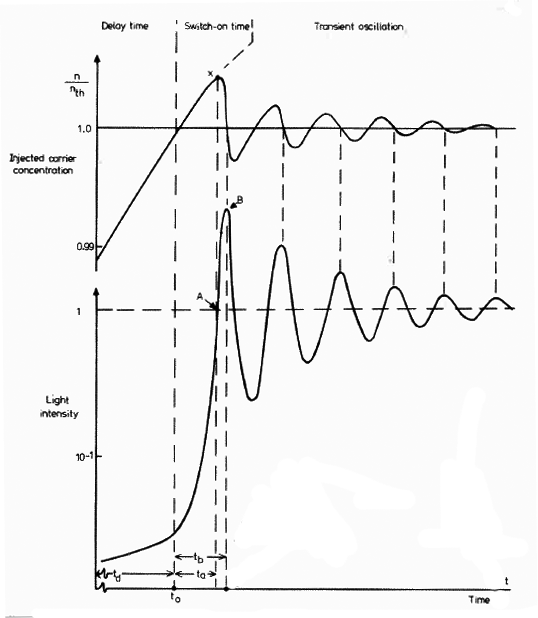
\includegraphics[scale=0.5]{LasPRelaxOsc}
  \caption{Time evolution of the carrier and photon population
    exhibiting relaxation oscillations}
  \label{fig:LasPRelaxOsc}
\end{figure}

% ---------------------------------------------------------------------
\paragraph{Circuitry and experimental setup}
 
As it was mentioned above FPGA is the source of voltage pulse driving
laser diode.  FPGA output pin has low output current and cannot drive
50 Ohm coaxial line directly.  To solve this problem there is buffer-1
in circuitry between the output pin of FPGA and 50 Ohm coaxial
line. It's CDCVF2310 Clock buffer and circuit is shown in
Fig.~\ref{fig:LasPBuf}.  To lower load of this buffer there is another
one buffer-2 before signal is delivered to SRD-unit.  Components of
SRD-unit are soldered as close to the modulation terminal of the laser
as possible. This prevents ringing due to mismatch and high frequency
we are dealing with. The duration of voltage pulse can be adjasted by
SRD diod bias voltage $V_s$. The amplitude of voltage pulse is fixed
and defined by the buffer-2 supply voltage $V_{dd}$.  Block view is
shown in Fig.~\ref{fig:LasPSRDunit}. Entire experimental setup is
shown in Fig.~\ref{fig:LasPSetup}.

\begin{figure}[!hbt]
  \centering
  \begin{tikzpicture} [auto,
    main/.style={rectangle,draw=black!50,fill=black!20,thick}, every
    label/.style={green}]

    \node [main] (FPGA) [label=above:$200MHz$] {FPGA}; \node [main]
    (BUF1) [right=of FPGA, label=below:$CDCVF2310$] {Buffer 1};
    \node [main] (BUF2) [right=of BUF1, label=below:$CDCVF2310$]
    {Buffer 2}; \node [main] (SRD) [right=of BUF2] {SRD unit}; \node
    [main] (LD) [right=of SRD, label=above:$FLD5F15CX$] {Laser};
    \node [main] (SRDB) [above=of SRD] {SRD bias control}; \node
    [main] (SCOPE1) [above=of LD, label=above:$TDS7104$] {Scope 1};
    \node [main] (SPECA) [below=of LD, label=above:$HP86140A$]
    {Spectrum analizer}; \node [main] (PD) [below=of LD]
    {Photodetector}; \node [main] (OPM) [below=of LD,
    label=above:$17XTF$] {Optical power meter}; \node [main]
    (SCOPE2) [below=of PD, label=above:$TX7854$] {Scope 2};

    \draw [->] (FPGA) to (BUF1); \draw [->] (BUF1) to (BUF2); \draw
    [->] (BUF2) to (SRD); \draw [->] (SRD) to (LD); \draw [->] (LD)
    to (PD); \draw [->] (LD) to (SPECA); \draw [->] (LD) to (OPM);
    \draw [->] (PD) to (SCOPE2); \draw [->] (SRD) to (SCOPE1); \draw
    [->] (FPGA) to (SCOPE2); \draw [->] (SRDB) to (SRD);
  \end{tikzpicture}
  \caption{Pulse mode experimental setup}
  \label{fig:LasPSetup}
\end{figure}

\begin{figure}
  \centering
  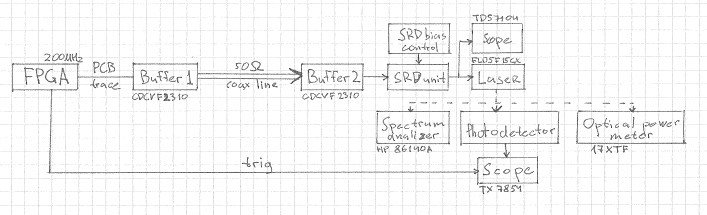
\includegraphics[scale=0.5]{LasPSetup}
  \caption{Pulse mode experimental setup}
  \label{fig:LasPSetp}
\end{figure}

\begin{figure}
  \centering
  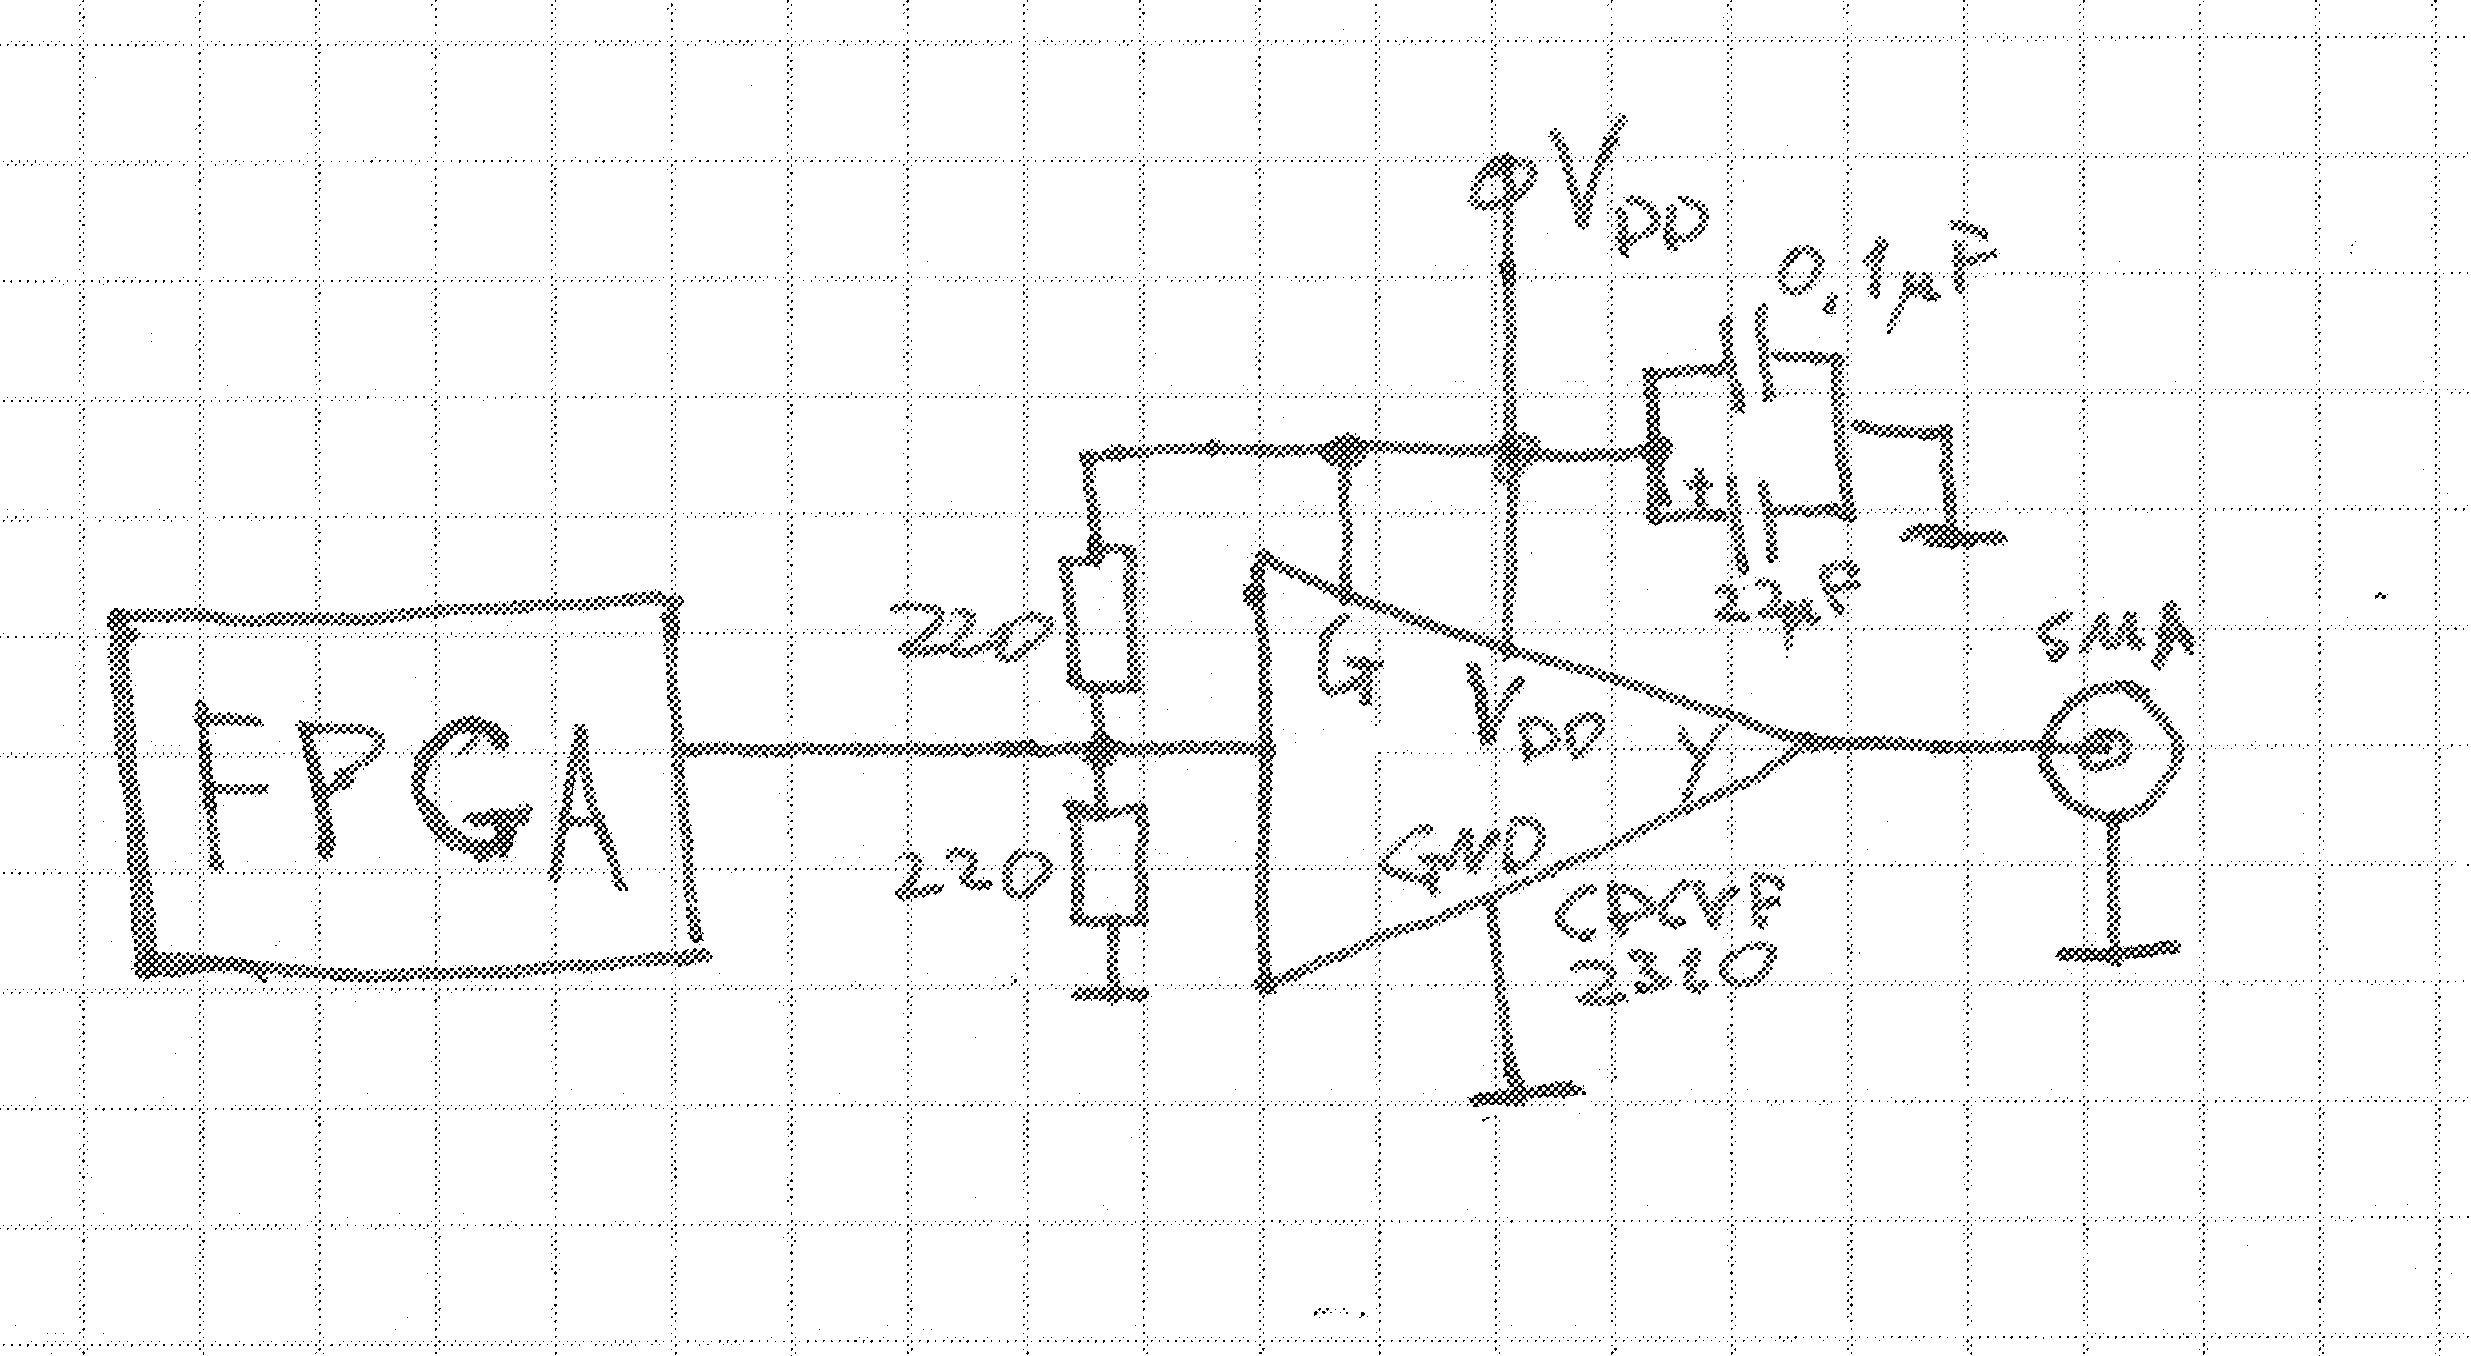
\includegraphics[scale=0.1]{LasPBuf}
  \caption{Buffer circuitry}
  \label{fig:LasPBuf}
\end{figure}

\begin{figure}
  \centering
  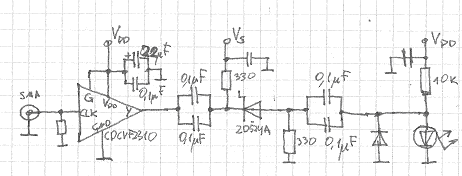
\includegraphics[scale=0.7]{LasPSRDunit}
  \caption{SRD unit circuitry}
  \label{fig:LasPSRDunit}
\end{figure}


% ---------------------------------------------------------------------
\paragraph{Experimental results}

Measured optical pulse FWHM width and average optical power on the
output of laser shown in Table\ref{tab:LasPExp}.  Isolating of one
optical cycle maded by adjacment of voltage pulse width.

\begin{table}[!hbt]
  \centering
  \begin{tabular}{|c|c|c|c|}
    \hline
    $V_s{,}V$ & $P_0{,\mu}W$ & $\pulse width{,}ps$ & {osc.}\\
    \hline
    0.024 & 21.8 & 111.3 & a,d \\
    \hline
    -0.058 & 43.5 & 105 & c \\
    \hline
    -0.134 & 77 & -- & c \\
    \hline
  \end{tabular}
  \caption{Pulsed mode}
  \label{tab:LasPExp}
\end{table}

Illustration of different pulses shape according to different SRD bias
voltage is shown on Fig.~\ref{fig:LasPOsc}\footnote{author apologise
  for low quality oscillogramms, but fast oscilloscope needed to
  characterize pulses shape is old analog one and has no output to
  printer}.  Oscillogramms $a$ and $d$ relate to the working
regime. Working regime is regime with optical pulse height equal to
$1/2$ of boundary regime shown on oscillogramm $b$. Oscillogramm $c$
illustrate regime with noticible second optical cycle.

\begin{figure}
  \centering
  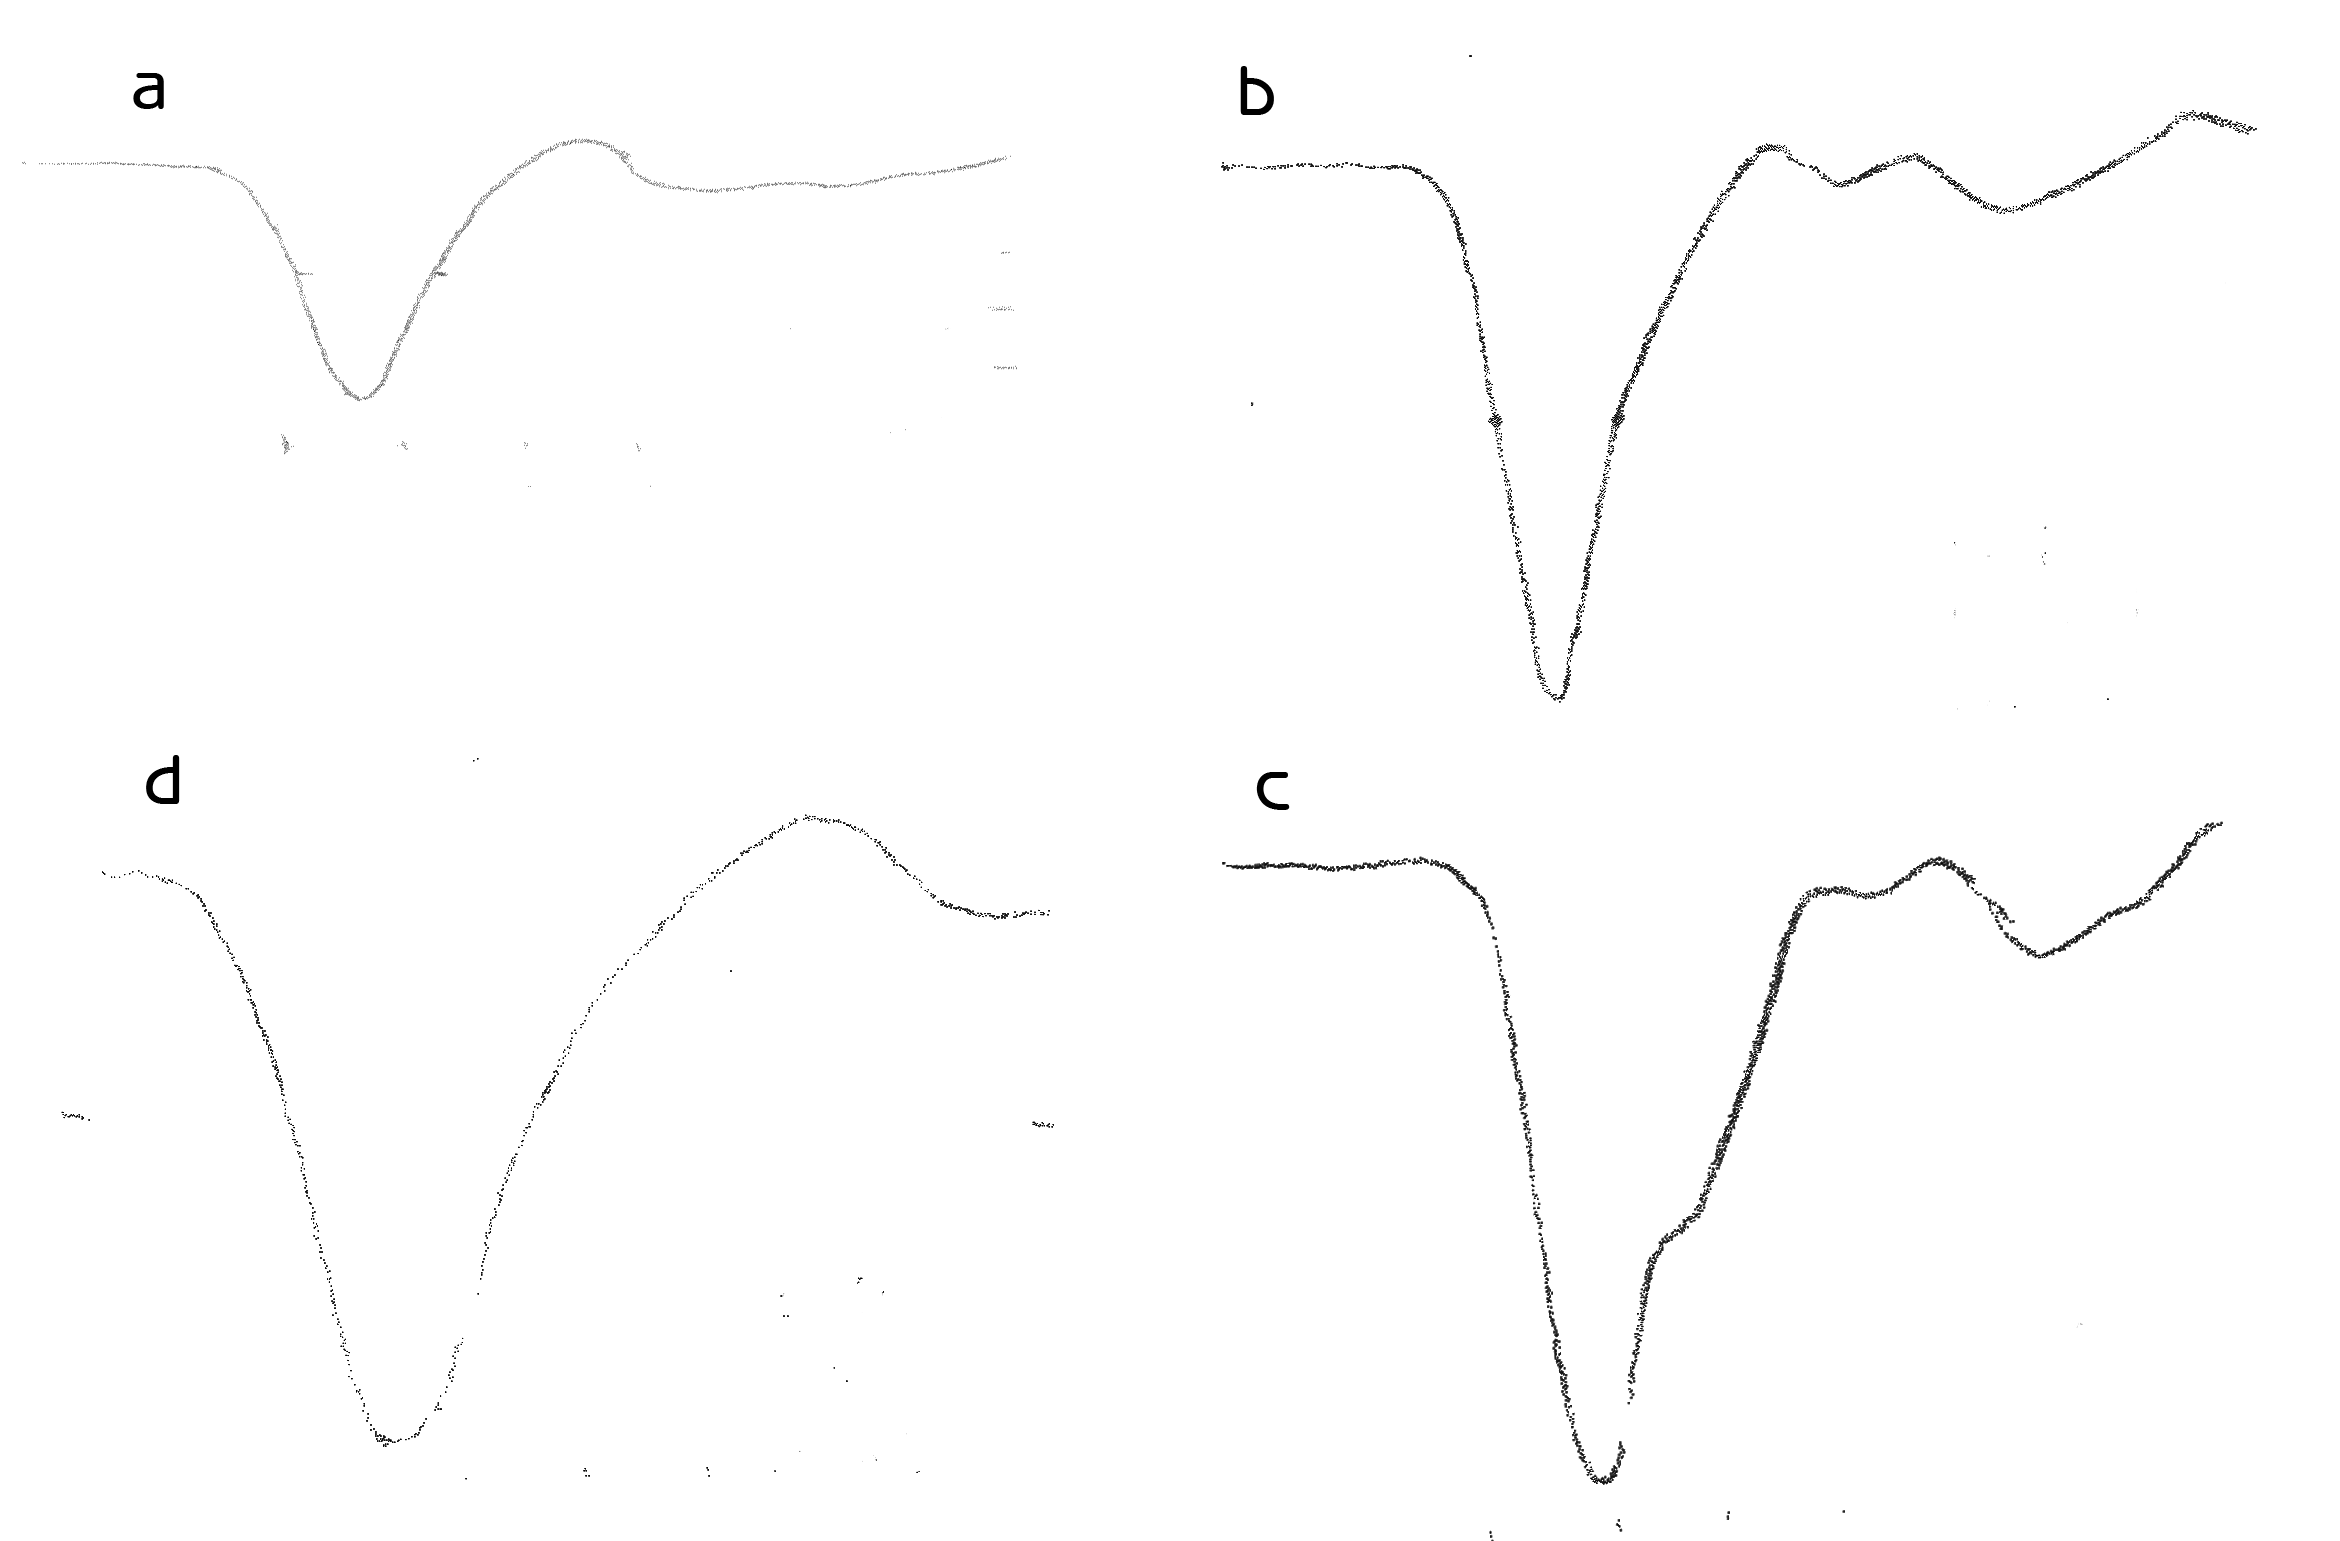
\includegraphics[scale=0.1]{LasPOsc}
  \caption{Pulses shapes}
  \label{fig:LasPOsc}
\end{figure}

% ---------------------------------------------------------------------
\subparagraph{Pulse power}

It's possible to calculate the energy in the optical pulse by
analyzing the average output power and pulse width on output of the
laser.

% ---------------------------------------------------------------------
\subparagraph{Pulse efficiency}

The energy of the optical pulse is proportional to the number of
photons.  The energy of $x$ photons in a pulse is given by
\begin{equation}
  n_{photon}=\frac{E_{o}}{h\cdot\nu}
\end{equation}
The pulse with the specified optical energy is passed through an
optical attenuator with a loss of $D dB$.  This determines the average
number of photons, called the pulse efficiency of the optical pulse
\begin{equation}
  \nu=\frac{n_{photon}}{10^{d/10}}
\end{equation}


% ---------------------------------------------------------------------
\subparagraph{Number of photons}

Number of photons in the optical pulse is Poisson distributed. The
parameters in the Poisson distribution is given by the pulse
efficiency of the attenuated laser pulse. The probability of $x$
photons in a pulse, $P(x)$, is given by
\begin{equation}
  P(x)= \frac{e^{-\eta}\cdot{\eta^x}}{x!}
\end{equation}
If the pulse efficiency is too large there is a higher probability of
more than one photon per pulse.

% ---------------------------------------------------------------------
\subparagraph{Jitter}

Arrival times of photons is distributed according to the shape of the
optical pulse. This causes a phase jitter. The maximum of the jitter
is given by the width of the optical pulse. Our pulse is about 100 ps
wide FWHM.

% ---------------------------------------------------------------------
\subsection{Intensity and phase modulation drivers}


%---------------------------------------------------------------------
\section{Software modules}

%---------------------------------------------------------------------
\subsection{Dataflow}

%---------------------------------------------------------------------
\subsection{FPGA internals}

%---------------------------------------------------------------------
\paragraph{Pseudo random number generator}